\subsection{Bitcrusher}
\label{subsec:desarrollo-bitcrusher}

\subsubsection{Descripción}
\label{subsec:desarrollo-bitcrusher-desc}
En la sección \fullref{subsec:intro-audio} se habló sobre dos medidas de audio digital que son quienes determinan la \textit{calidad} del sonido: la frecuencia de muestreo (\textit{sampling rate}) y la resolución de la muestra (\textit{bit rate}). El efecto \textbf{bitcrusher} provoca una distorsión de la señal original, reduciendo tanto el muestreo (se toma en la señal húmeda una de cada cierta cantidad de muestras de la señal original, \textbf{downsampling}) como la cantidad de bits con la que se puede expresar cada muestra (\textbf{quantization}).

Los resultados de este efecto muchas veces hacen recordar a la música de los primeros juegos de consola (también conocidas como \textbf{chiptunes}), pues eran generadas con chips de 8 bits.

En la siguiente imagen, puede apreciarse cómo el efecto distorsiona la señal original (onda superior).

\begin{figure}[H]
    \centering
    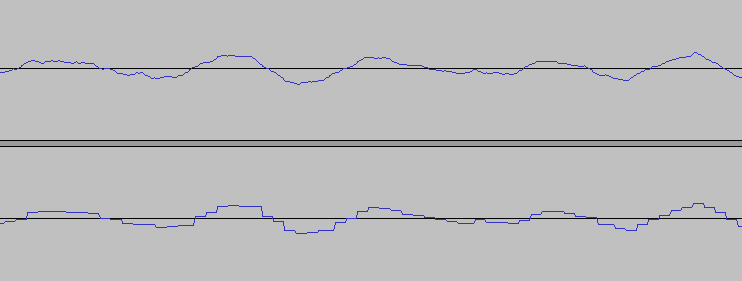
\includegraphics[scale=0.6]{imagenes/bitcrusher-signal.png}
    \caption{Señal superior: original. Señal inferior: al aplicar el efecto.}
    \label{fig:bitcrusher-signals}
\end{figure}


\vspace{\baselineskip}

Los resultados de la comparación entre las versiones en \textbf{C} y \textbf{ASM} de este algoritmo se verán en la sección \fullref{subsec:resultados-bitcrusher}, y el análisis en \fullref{sec:analisis}.

\subsubsection{Pseudocódigo}
\label{subsec:desarrollo-bitcrusher-code}

\lstset{language=C}
\begin{lstlisting}[frame=single]
Argumentos: bits, freq
step = 1/2^(bits);
phasor = last = 0;
normFreq = freq/archivoEntrada.samplerate

Para cada muestra
  phasor = phasor + normFreq;
  if (phasor >= 1.0) { 	
  // downsampling, tomo 1 muestra de cada cierta cantidad
    phasor = phasor - 1.0; 
    last = step * floor( input(i)/step + 0.5 );
    // quantization, reduzco la calidad 
  }

  dataBuffOut.canalDerecho = last
  dataBuffOut.canalIzquierdo = dataBuffIn.muestraCicloActual

\end{lstlisting}

\subsubsection{Comando}
\label{subsec:desarrollo-bitcrusher-call}

\underline{\textbf{C}}:
\begin{center}
 \textit{./main INFILE OUTFILE -}
\end{center}

\underline{\textbf{ASM}}:
\begin{center}
 \textit{./main INFILE OUTFILE -}
\end{center}

\begin{itemize}
 \item \textit{bits}: argumento con rango entre 1 y 16. Es la cantidad de bits que se pueden utilizar para el valor de cada muestra.
 \item \textit{freq}: argumento con rango entre 2048 y 11025Hz. Es la frecuencia de sampleo de la señal húmeda.
\end{itemize}
 
 
